\documentclass[a4paper]{article}
\usepackage[margin=2cm]{geometry}
\usepackage[english]{babel}
\usepackage[utf8]{inputenc}
\usepackage[T1]{fontenc}
\usepackage{times}
\usepackage{float}
\usepackage{listings}
\usepackage[pdftex]{graphicx}
\usepackage{epstopdf}
\usepackage{pdfpages}
\usepackage{color}
\usepackage[pdftex,colorlinks=true,citecolor=black,
            pagecolor=black,linkcolor=black,menucolor=black,
            urlcolor=black]{hyperref}
\usepackage{eufrak}
\usepackage{amsmath}
\usepackage{amsbsy}
\usepackage{eucal}
%\usepackage{subfigure}
\usepackage{longtable}
\usepackage{url}
\urlstyle{same}

\usepackage{natbib}

\parindent 0mm
\parskip 3mm

\newcommand*\mean[1]{\bar{#1}}

\pdfinfo{            
          /Title      (T-61.5140 Machine Learning: Advanced Probabilistic Methods Project)
          /Author     (Ville Sillanpää, Lauri Viitanen)
          /Keywords   ()
}

\title{Classify the glass samples using Gaussian Mixture Models (GMM)}
\author{Ville Sillanpää, k84338 - Lauri Viitanen, 338853 \\ 
       {\it ville.sillanpaa@aalto.fi} -
       {\it lauri.viitanen@aalto.fi}}

\begin{document}
\maketitle
\clearpage

%\begin{figure}[]
%	\includegraphics[]{all_338853_2001.pdf}
%\end{figure}

\section{Introduction}

In this project we analyze a glass data set using both unsupervised and
supervised machine learning approaches. The glass dataset [1] has been
provided by the US Forensic Science Service and is available for download from
the UCI machine learning repository. The dataset consists of samples for 6
types of glass (class label 4 is missing in the current data set); defined in
terms of their oxide content (i.e. Na, Fe, K, etc). In particular, the dataset
contains 214 samples characterized by 9 features and the samples have been
categorized into 6 different classes of glass.

\par
The goal of the project is to classify the glass samples using Gaussian
Mixture Models (GMM) in unsupervised and supervised approaches. In the
unsupervised approach we use GMMs to find clusters from the full data set and
compare the clustering results with the ground-truth class labels that are
provided with the data set. In the supervised approach we fit a separate GMM
for each class label and evaluate the classification performance using the
fitted models on the test set. The dataset has been randomly divided into
training (75 \%) and test sets (25 \%) keeping an equal proportion of different
class instances in the training and test sets. In addition, we compare the
performance of the GMM model with the k-nearest neighbors classifier.

\section{Methodology}

This section describes the methods used in the analysis. Unsupervised and supervised approaches are described in their own subsections. Unsupervised classification was done using Gaussian Mixture Model with Dirichlet Process prior (sometimes referred to as Infinite Gaussian Mixture model). Supervised classification was done using Gaussian Mixture Model (GMM) with no prior distributions for model parameters.

\subsection{Unsupervised Approach}

Dirichlet Process Gaussian Mixture Model (DP-GMM) was selected for unsupervised classification, as it does not require user to specify the number of clusters beforehand. Instead, the model allows structure of data define how many clusters the model ends up with. This is a major asset when compared to traditional GMM,  as it is often difficult to assess how many clusters an 'optimal' model has. This property is especially of use in this analysis, where we don't really know anything about the data beforehand. 

Specification of the model and algorithm is presented in appendix of this document. Algorithm for inferring the model is a Gibbs sampling scheme, that goes through all data points in turn, takes their previous cluster label status off, finds each point a new cluster label and then learns cluster-specific parameters for each cluster (clusters are multivariate normal densities). Finding a new cluster label is done in so that each data point can either get assigned to some pre-existing cluster or a new cluster can be generated altogether.

  
\subsection{Supervised Approach}

In the supervised approach, the Gaussian mixture model is fitted to every
class label separately. The model complexities range from 2 to 10 components.
Class label 4 has no samples in the training data, class label 6 has only six
samples and class label 5 has nine samples, meaning that using more than nine
classes already drops the number of class labels from seven to four. Only
classes 1 and 2 have more than 21 samples.

\par
The GMM is fitted to the training data using the Expectation-Maximization (EM)
algorithm. The training halts after 200 iterations or if the log likelihood
has not changed enough (0.001 units) during the past few iterations (five).
The resulting fitted Gaussians are then applied to the test data of the same
classes, producing the log likelihood of the test data being produced by the
fitted GMM.

\par
The class of the GMM that is most likely to produce a data point in the test
set is selected as the class of the test data point. This is repeated for all
test data points first for all six GMM's with two clusters, then with all six
GMM's with three clusters etc., until for every cluster count the test data is
labeled. The resulting estimated labels are then compared to the known true
labels of the test data and a confusion matrix is calculated.

\section{Results}

This section describes the results. Results from unsupervised and supervised analysis are presented in their own subsections. As a summary of results from unsupervised approach, we say that the model was able to identify only one cluster well. With remaining clusters the model had more mixed results. Details that lead to this conclusion are presented in the next paragraph. For supervised method, labels 1, 3 and 7 were recognized with more than 50 \% accuracy, but the performance of GMM-EM algorithm compared to kNN, $ k = 1 $, is not very good.

\subsection{Unsupervised Approach}

\par
A Gibbs sampling Markov chain of 5000 observations was ran. Below is the distribution of number of clusters estimated from the last 2500 samples of the chain.

\begin{figure}[H]
	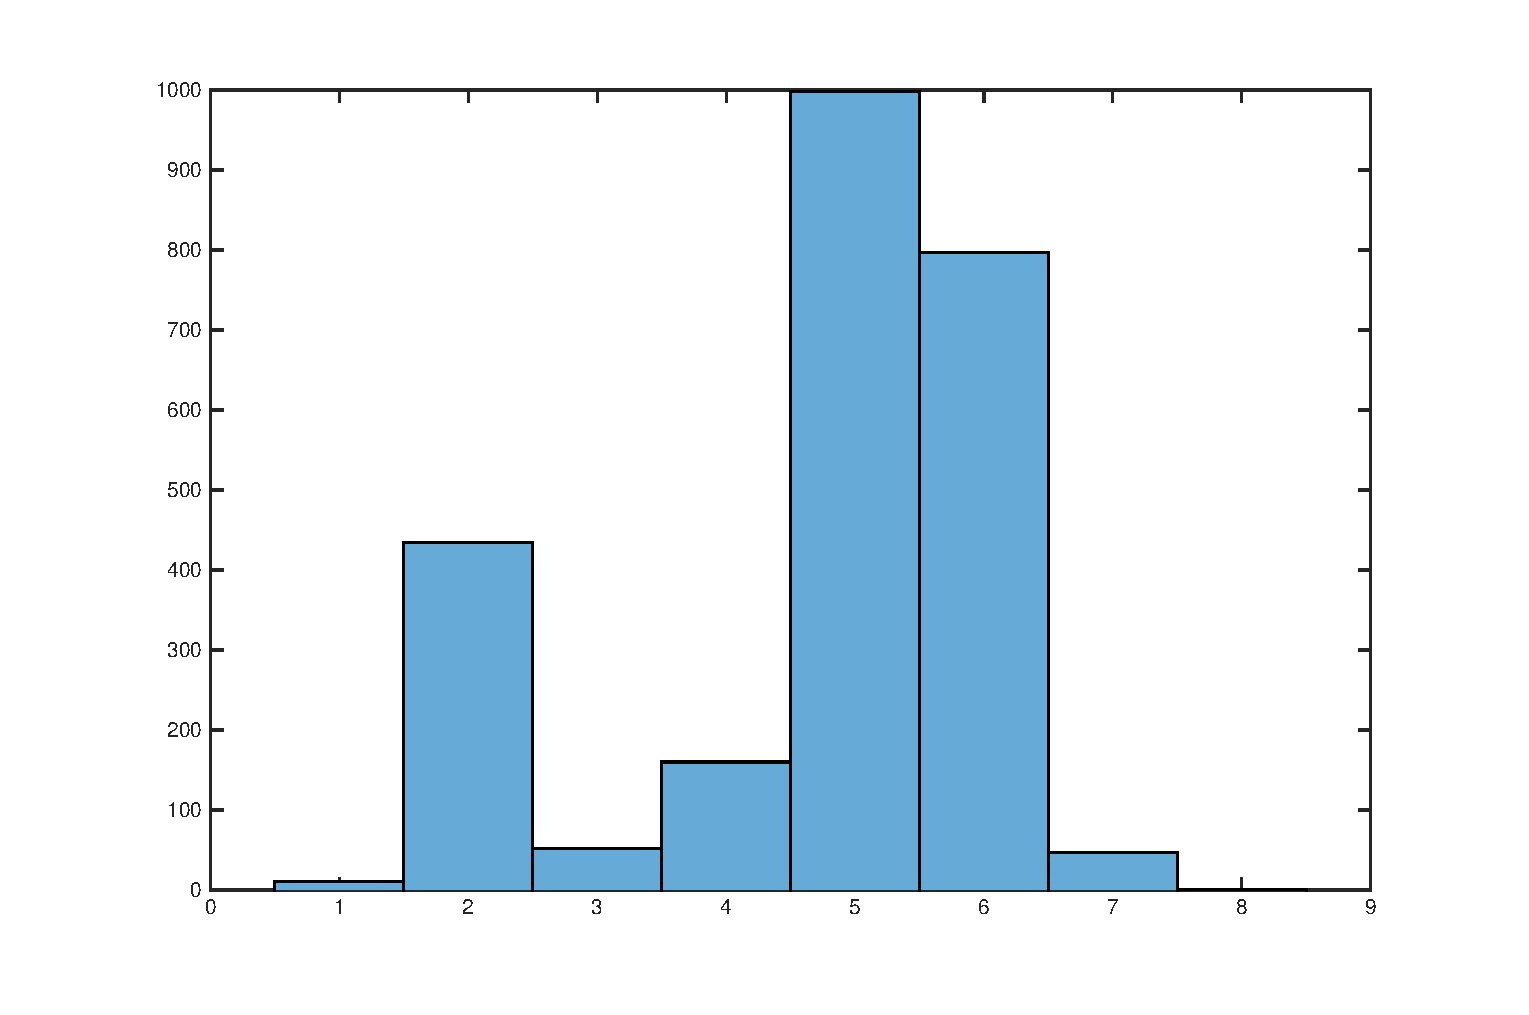
\includegraphics[trim={2cm 1cm 2cm 1cm},clip,scale=0.56]{k_dist_5000.eps}
	\caption{Cluster amount distribution of data from 2500 samples}
	\label{k_dist}
\end{figure}

As we can see from figure \ref{k_dist}, typically our model found 5 clusters with 6 and 2 being quite likely outcomes as well. The ground truth was that there were 6 clusters. So it seems that the model was unable to characterize this data in a manner that would  unambiguously reflect this.

Reasons for this become evident when we visualize the results. Below is a scatter plot from one of the runs. The visualization was produced with multidimensional scaling. PCA was tried first, but since the first two components explained only two thirds of variation, we chose to to MDS instead. 

\begin{figure}[H]
	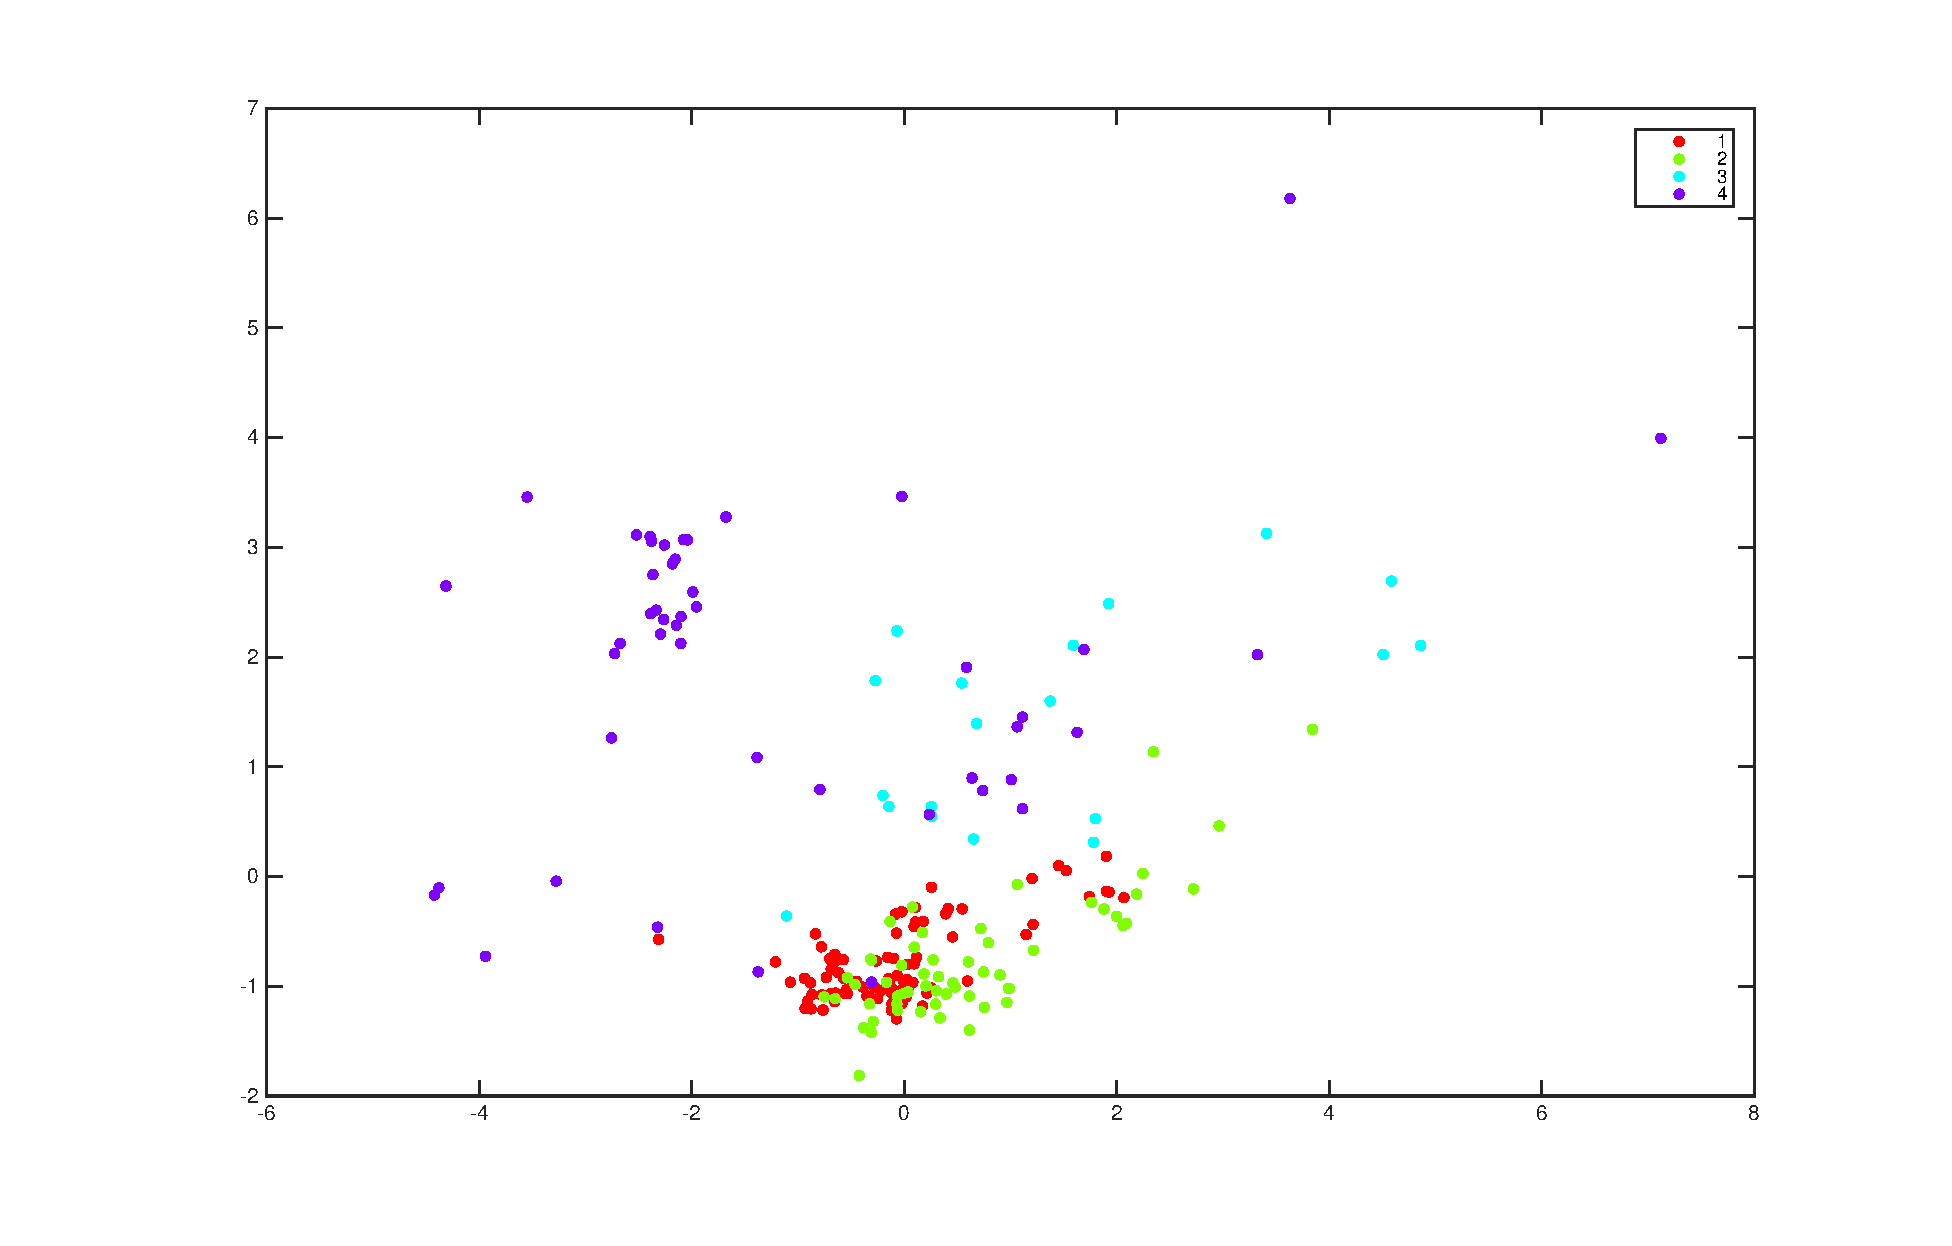
\includegraphics[trim={3.5cm 1.5cm 3cm 1.3cm},clip,scale=0.45]{5000_normalized_data_1.eps}
	\caption{MDS of data with colors representing cluster labels found with DP-GMM}
	\label{mds_unsupervised}
\end{figure}

As you can see from figure \ref{mds_unsupervised}, two dense clouds of points have been identified to belong to three clusters. This result was very common in runs that found more than two clusters. The runs that found only two clusters saw the two dense clouds as two separate clusters.

 The points that are spread more sparsely were assigned to various clusters in various runs. Based on inspection of few samples the labeling of these data points was very arbitrary. Hence based on this model it is difficult to say what clusters the sparse points belong to or that how many true labels these sparse points represent.

To see how our model compares with ground truth, let's look at MDS-visualization with points given color codes based on true labels.

\begin{figure}[H]
	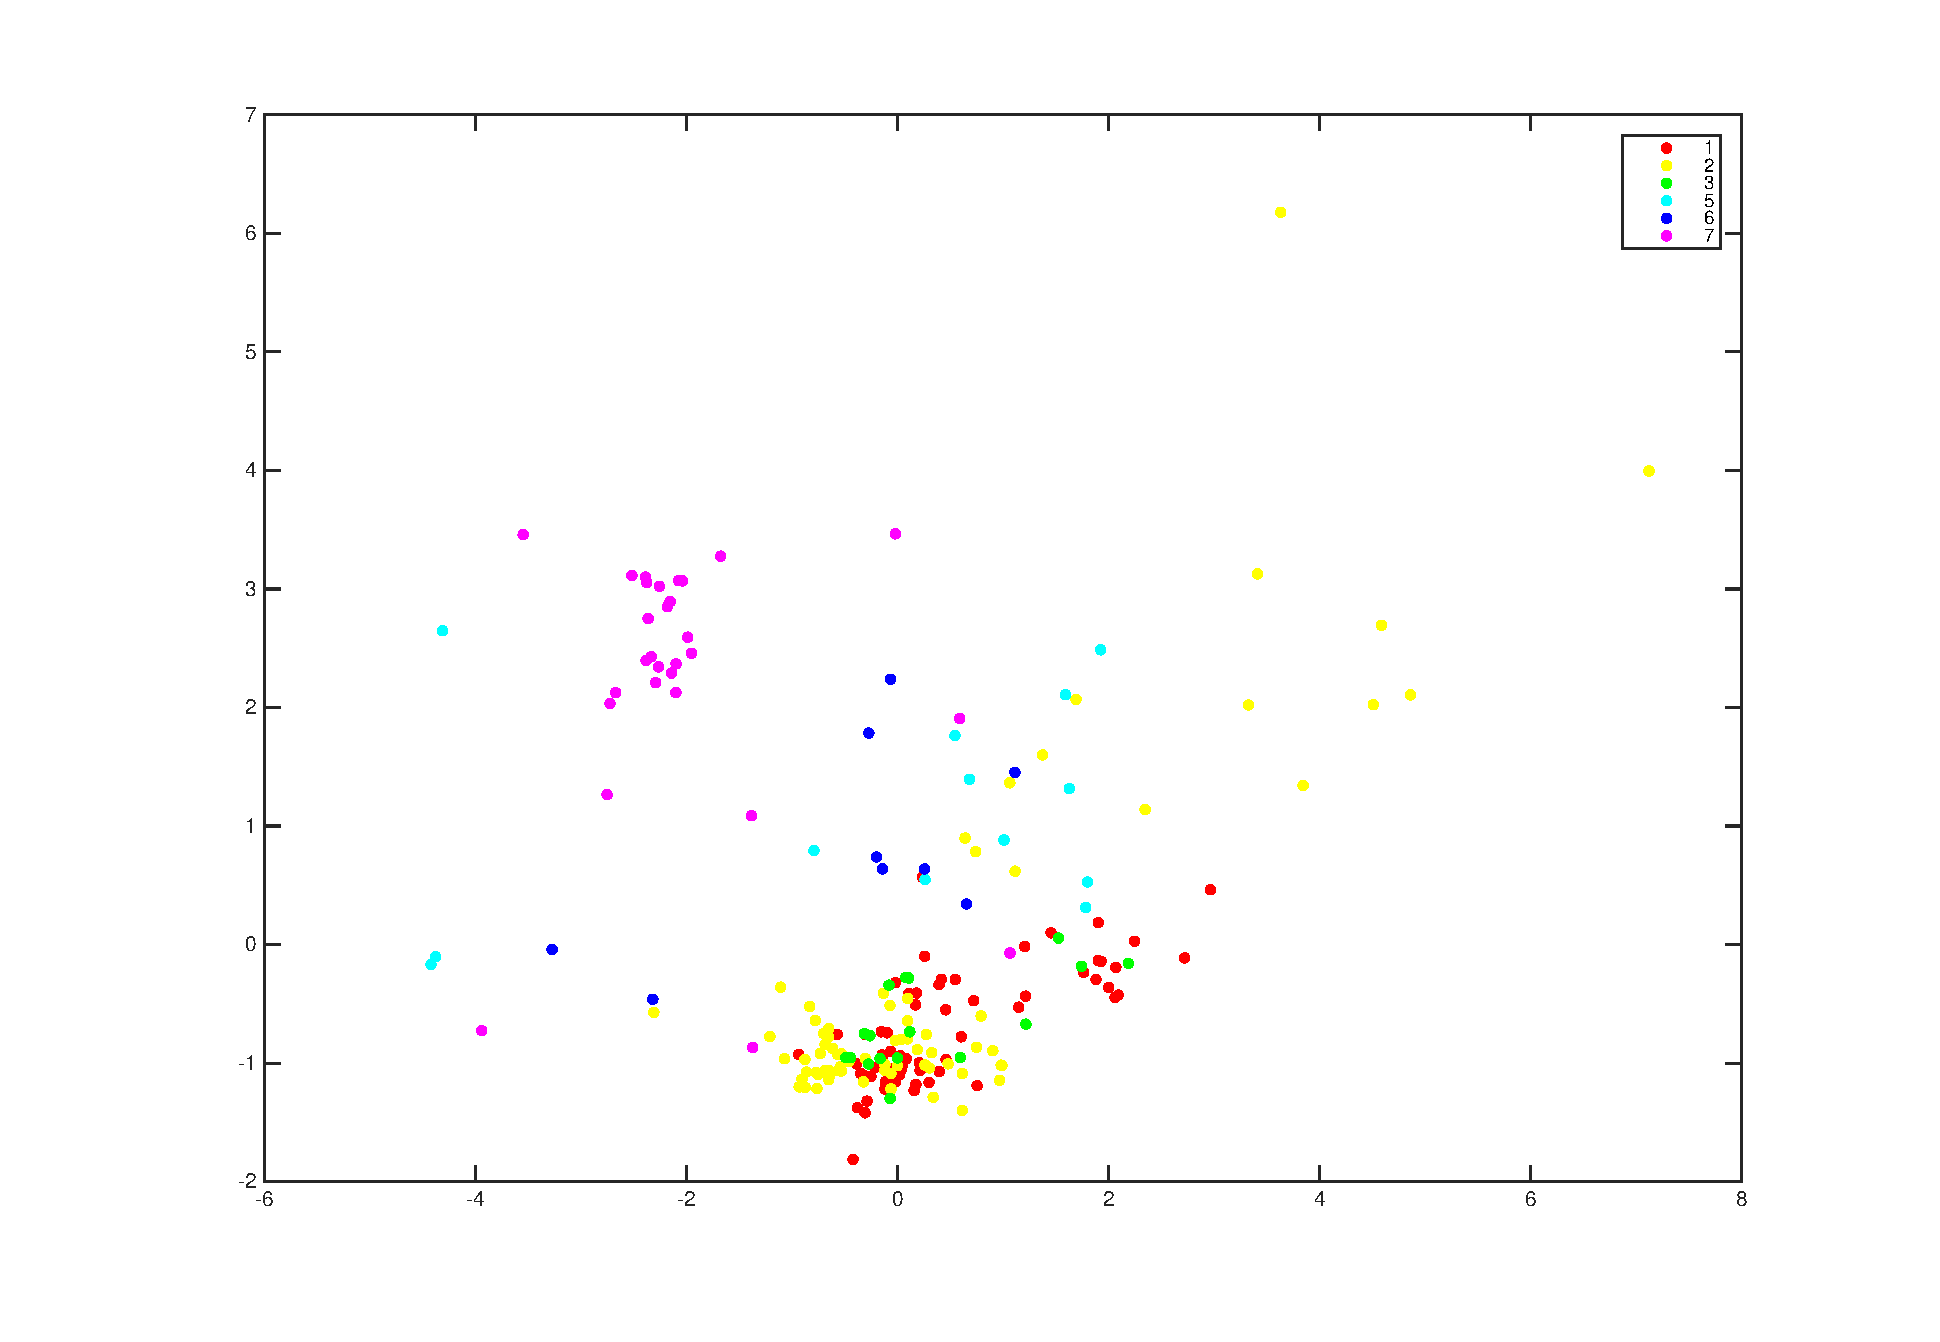
\includegraphics[trim={3.5cm 1.5cm 3cm 1.3cm},clip,scale=0.45]{MDS_true_labels.eps}
	\caption{Visualization of data with true labels as color codes}
	\label{true_labels}
\end{figure}

As we can see from figure \ref{true_labels}, the lower dense region is more overlapping than what our model usually predicts. Moreover,  quite a few of the more sparse points seem to belong to a label that is very densely concentrated in the bottom (yellow). Apparently the sparse region contains observations from two additional labels. They seem to overlap so much that it is difficult to see how a Gaussian mixture model would be able to find these two clusters correctly. Model and ground truth seem to agree the most about the upper dense cloud (label 7 in real data). 

\subsection{Supervised Approach}

The listing below shows how the GMM performed.
All the confusion matrices are very similar with each other. No matter the
number of clusters, data points in classes 2, 5 and 6, in that order, were the
most difficult to classify. Classes 7, 3 and 1, in that order, were found most
reliably. This observation agrees with the results gained from the unsupervised
approach, where data points in class 7 were found to belong to a single cluster
distinct from the rest of the data. Clusters 1 and 2 are the largest and
overlap so heavily that classification method based on comparing normal
distribution densities tends to systematically favor one of the two
distributions i.e. the one which has more clustered data points. This behaviour
could be avoided by using Student's t-distribution or other long tailed
distribution instead of Gaussians for better robustness against outliers.

\begin{verbatim}
Mean over all cluster counts
0.63 0    0.37 0    0    0   
0.25 0.18 0.47 0.04 0.05 0.01
0.25 0    0.75 0    0    0   
0    0.44 0    0.28 0.22 0.06
0    0.74 0    0    0.26 0   
0    0.13 0    0.03 0.07 0.78
\end{verbatim}

\iffalse
\begin{verbatim}
        Two clusters                  Three clusters
0.53 0    0.47 0    0    0      0.65 0    0.35 0    0    0   
0.22 0.17 0.50 0    0.11 0      0.33 0.17 0.39 0    0.11 0   
0.25 0    0.75 0    0    0      0.25 0    0.75 0    0    0   
0    0.50 0    0.25 0.25 0      0    0.50 0    0.25 0.25 0   
0    1.00 0    0    0    0      0    0.67 0    0    0.33 0   
0    0    0    0    0.25 0.75   0    0.13 0    0    0.13 0.75

       Four clusters                   Five clusters
0.65 0    0.35 0    0    0      0.65 0    0.35 0    0    0   
0.39 0.17 0.33 0    0.11 0      0.22 0.17 0.50 0    0.11 0   
0.25 0    0.75 0    0    0      0.25 0    0.75 0    0    0   
0    0    0    0.25 0.75 0      0    0    0    0.25 0.75 0   
0    0    0    0    1.00 0      0    0    0    0    1.00 0   
0    0.13 0    0    0.13 0.75   0    0.13 0    0    0.13 0.75

        Six clusters                  Seven clusters
0.65 0    0.35 0    0    0      0.65 0    0.35 0    0    0   
0.22 0.17 0.50 0.11 0    0      0.22 0.17 0.50 0.11 0    0   
0.25 0    0.75 0    0    0      0.25 0    0.75 0    0    0   
0    0.50 0    0.50 0    0      0    0.50 0    0.50 0    0   
0    1.00 0    0    0    0      0    1.00 0    0    0    0   
0    0.13 0    0.13 0    0.75   0    0.25 0    0    0    0.75

      Eight clusters                   Nine clusters
0.65 0    0.35 0    0    0      0.65 0    0.35 0    0    0   
0.22 0.17 0.50 0.11 0    0      0.22 0.22 0.50 0    0    0.06
0.25 0    0.75 0    0    0      0.25 0    0.75 0    0    0   
0    0.50 0    0.50 0    0      0    0.75 0    0    0    0.25
0    1.00 0    0    0    0      0    1.00 0    0    0    0   
0    0.13 0    0.13 0    0.75   0    0.13 0    0    0    0.88

        Ten clusters            Mean over all cluster counts
0.65 0    0.35 0    0    0      0.63 0    0.37 0    0    0   
0.22 0.22 0.50 0    0    0.06   0.25 0.18 0.47 0.04 0.05 0.01
0.25 0    0.75 0    0    0      0.25 0    0.75 0    0    0   
0    0.75 0    0    0    0.25   0    0.44 0    0.28 0.22 0.06
0    1.00 0    0    0    0      0    0.74 0    0    0.26 0   
0    0.13 0    0    0    0.88   0    0.13 0    0.03 0.07 0.78
\end{verbatim}
\fi

\par
The supervised GMM has not very large difference between the performance of
GMM's with different cluster count. They mean of correct classifications for
each GMM is between 40 \% and 50 \%, but GMM's with four or five clusters seem
to perform systematically better than the rest. GMM's with 2, 9 or 10 clusters
performed clearly the worst. This is most probably the result of finding the
best balance between generalization (less than four clusters) and fit (more
than five clusters).

\begin{verbatim}
 kNN confusion matrix, k = 1
0.88 0.06 0.06 0    0    0   
0.06 0.83 0    0    0.11 0   
0.50 0    0.50 0    0    0   
0    0.50 0    0.50 0    0   
0    0    0    0    1.00 0   
0.13 0.13 0    0    0    0.75
\end{verbatim}

\par
Finally, the GMM's performance is benchmarked against kNN clustering, $ k = 1 $
and the distance measure was Euclidean. The trained algorithm's confusion
matrix upon test data is shown below. The average performance (74 \% of
classifications were correct) is significantly better than for GMM's with any
number of clusters. Clusters 1 and 2, the ones with most data, and 6 and 7,
were predicted with greatest accuracy. 

\par
It seems that kNN is clearly superior for the glass dataset classification task. This is most likely because most of the clusters are very overlapping and - at least according to MDS visualizations - lack the sort of round and uniform structure Gaussian Mixture Models assume. Unlike GMM, kNN only uses few surrounding points in its inference and does not use any other information than distance. Thus it performs well in classification tasks, where overlap between several labels is characterized by some level of closeness between individual data points of same label. As shown in Figure \ref{c_equals_k}, this kind of overlap can be seen between 1 and 2. 

%\section{Discussion}

%Neither the unsupervised DP-GMM or the supervised GMM-EM found all six labels,
%nor succeeded in classification. Most common number of labels that the methods
%found was five, with is rather well considering that two of the classes
%cover over two thirds of the data, and some labels are represented with only
%a few data points. Clustering based on round Gaussian distributions is not
%a very good tool for the dataset at hand. The kNN algorithm, $ k = 1 $,
%outperforms both methods by clear margin. 

\section{References}
\par
[1] Dataset http://archive.ics.uci.edu/ml/datasets/Glass+Identification
\par
[2] F. Wood, S.Goldwater \& M.Black A Non-Parametric Bayesian Approach to Spike Sorting, Department of Computer Science \& Department of Cognitive and Linguistic Sciences, Brown University, Providence, RI, USA, 2006

[3] Code for algorithm used in unsupervised approach http://www.gatsby.ucl.ac.uk/~fwood/code.html

\section{Appendix}

\subsection{Model description for GMM with Dirichlet  process prior}

 Model description below is a brief adaptation from Wood et al. (2006) [2]. For more elaborate description of model with appropriate referencing to previous work leading into this model specification, see  Wood et al(2006) [2]. 

Model assumes that our dataset comes from the following generative model:

\begin{equation}
\begin{aligned}
c_i | \pi \sim Multinomial(\cdot | \pi) \\
y_i | c_i = k, \theta \sim N(\cdot | \theta_k)
\end{aligned}
\end{equation}

Where $C=\{c\}\}^{N}_{i=1}$ indicate which class each observation belongs to, $\theta=\{\theta_k\}^K_{k=1}=\{\mu, \Sigma_{k}\}$ are parameters that characterize each class distribution, $Y=[y_i, ... y_N]$ are observations and $\pi=\{\pi_k\}^K_{k=1}=P(c_i=k)$ are class membership distribution parameters.

We model this data generation process with following model (assuming $K$, the number of classes, is finite):

\begin{equation}
\begin{aligned}
\pi | \alpha \sim Dirichlet(\cdot | \frac{\alpha}{K}, ... , \frac{\alpha}{K}) \\
\theta \sim G_0
\end{aligned}
\end{equation}

Where $\theta \sim G_0$ is shorthand for

\begin{equation}
\begin{aligned}
\Sigma_{k} \sim Inverse-Wishart_{v0}(\Lambda^{-1}_0) \\
\mu \sim N(\mu_0, \Sigma_{k}/\kappa_0)
\end{aligned}
\end{equation}

Parameters of prior distributions Normal, Inverse-Wishart and (symmetric) Dirichlet encode our beliefs about parameters of the system. Under this model posterior distribution is

\begin{equation}
\begin{aligned}
P(C, \theta, \pi, \alpha | Y) \\
\propto P(Y | C, \theta,) P(\theta | G_0) \prod_{i=1}^{N} P(C_i | \pi) P(\pi | \alpha) P(\alpha)
\end{aligned}
\end{equation}

The idea is to sample from this distribution assuming that $K \rightarrow \infty$, which means that there are potentially infinite number of classes and that our finite data manifests a finite but unknown amount of them. The sampling is done using Gibbs sampling, which is possible because our prior distributions are all conjugate. Below are the conditional distributions that we sample from sequentially. See Wood (2006) for more detailed derivations and references:

\begin{equation}
\begin{aligned}
P(\theta | C, \pi, \alpha, \theta_{-k}, Y) \\
\propto  \prod_{c_i=k} P(y_i | c_i, \theta_{-k}) P_{G_0}(\theta_{-k})
\end{aligned}
\label{gauss_theta}
\end{equation} 

\begin{equation}
\begin{aligned}
P(c_i = k | C_{-i}, \pi, \alpha, \theta, Y) \\
\propto P(y_i | c_{-i}, \theta) P(c_i | C_{-i})
\end{aligned}
\label{c_equals_k}
\end{equation} 

\begin{equation}
\begin{aligned}
P(c_i | C_{-i}) =\\
\begin{cases}
\frac{m_k}{i-1+\alpha}, & \text{if } k \leq K_{+} \\
\frac{m_k}{i-1+\alpha}, & \text{if } k \geq K_{+}
\end{cases}
\label{crp}
\end{aligned}
\end{equation} 

Where $m_k$ is the number of observations in class $k$.

  \par
  Sample from this model is cluster membership status to all data points and distribution parameters to each existing cluster. The idea in the sampler is to go through all data points in turn, take their class status off and then sample a new class status to them from \ref{c_equals_k} with \ref{crp} allowing that a new cluster can be generated. If new cluster was generated, sample parameters to it from $G_0$. After this sample $\theta$ using \ref{gauss_theta}. This is done until log-likelihood of the model no longer increases substantially (which means that our samples are most likely from posterior and not from some intermediary state of the Markov Chain).
  
  The sampler we used was written by Wood (2006) and is available online [3]. This sampler also treats $\alpha$ as a random variable, and samples it for \ref{crp} from Gamma-distribution using Metropolis sampling.
  
  We used prior parameters Wood's algorithm had by default. So our prior distributions are $N(0, \Sigma_k / 1,), Inverse-Wishart_{1}(diag(0.3))$, where $diag(0.3)$ is a diagonal matrix with $0.3$ on diagonal. 
  
  We ran into problems in initial testing runs, as the algorithm did not seem to find more than 1 cluster for the entire data. As this seemed wrong, we centered each variable to 0 and scaled their variance to 1. While we don't know the root cause for the problems, we guess that it was due to the choice of priors (and some of our variables being quite far away from them). We chose this approach rather than rethinking the priors because it was more convenient to do.



%\begin{equation}
%\begin{aligned}
%	r[n] &= h[n] * s[n] \leftrightarrow
%		R(e^{j\omega}) = H(e^{j\omega})S(e^{j\omega}) \\
%	r[n] &= \sum_{k=-\infty}^{\infty} h[k]s[n-k] \\
%\end{aligned}
%\end{equation}

%Figure \ref{fig:100_104} shows combinations of these numbers

%\begin{figure}[H]
%	\includegraphics[scale=0.67]{m100_115_b.eps}
%	\caption{The amplitude response both in linear and logarithmic
%		(decibel) scale.}
%	\label{fig:100_115_b}
%\end{figure}

%\begin{center}
%\begin{tabular}{ c c c c }
%	                 & $f$, $[f] = Hz$ & $\omega$, $[\omega] = rad/sample$ & $W$ \\
%	passband cut-off & $f_p \approx 3000$ & $\omega_p \approx 0.6*pi $ & $W_p \approx 0.6 $ \\
%\end{tabular}
%\end{center}

%\clearpage
%\appendix
%
%\clearpage
%\section*{Appendix A}\label{code:asdf}
%
%Matlab code for asdf.
%
%\lstinputlisting{asdf.m}
%
\end{document}
